\documentclass[twoside]{book}

% Packages required by doxygen
\usepackage{fixltx2e}
\usepackage{calc}
\usepackage{doxygen}
\usepackage[export]{adjustbox} % also loads graphicx
\usepackage{graphicx}
\usepackage[utf8]{inputenc}
\usepackage{makeidx}
\usepackage{multicol}
\usepackage{multirow}
\PassOptionsToPackage{warn}{textcomp}
\usepackage{textcomp}
\usepackage[nointegrals]{wasysym}
\usepackage[table]{xcolor}

% Font selection
\usepackage[T1]{fontenc}
\usepackage[scaled=.90]{helvet}
\usepackage{courier}
\usepackage{amssymb}
\usepackage{sectsty}
\renewcommand{\familydefault}{\sfdefault}
\allsectionsfont{%
  \fontseries{bc}\selectfont%
  \color{darkgray}%
}
\renewcommand{\DoxyLabelFont}{%
  \fontseries{bc}\selectfont%
  \color{darkgray}%
}
\newcommand{\+}{\discretionary{\mbox{\scriptsize$\hookleftarrow$}}{}{}}

% Page & text layout
\usepackage{geometry}
\geometry{%
  a4paper,%
  top=2.5cm,%
  bottom=2.5cm,%
  left=2.5cm,%
  right=2.5cm%
}
\tolerance=750
\hfuzz=15pt
\hbadness=750
\setlength{\emergencystretch}{15pt}
\setlength{\parindent}{0cm}
\setlength{\parskip}{3ex plus 2ex minus 2ex}
\makeatletter
\renewcommand{\paragraph}{%
  \@startsection{paragraph}{4}{0ex}{-1.0ex}{1.0ex}{%
    \normalfont\normalsize\bfseries\SS@parafont%
  }%
}
\renewcommand{\subparagraph}{%
  \@startsection{subparagraph}{5}{0ex}{-1.0ex}{1.0ex}{%
    \normalfont\normalsize\bfseries\SS@subparafont%
  }%
}
\makeatother

% Headers & footers
\usepackage{fancyhdr}
\pagestyle{fancyplain}
\fancyhead[LE]{\fancyplain{}{\bfseries\thepage}}
\fancyhead[CE]{\fancyplain{}{}}
\fancyhead[RE]{\fancyplain{}{\bfseries\leftmark}}
\fancyhead[LO]{\fancyplain{}{\bfseries\rightmark}}
\fancyhead[CO]{\fancyplain{}{}}
\fancyhead[RO]{\fancyplain{}{\bfseries\thepage}}
\fancyfoot[LE]{\fancyplain{}{}}
\fancyfoot[CE]{\fancyplain{}{}}
\fancyfoot[RE]{\fancyplain{}{\bfseries\scriptsize Generated by Doxygen }}
\fancyfoot[LO]{\fancyplain{}{\bfseries\scriptsize Generated by Doxygen }}
\fancyfoot[CO]{\fancyplain{}{}}
\fancyfoot[RO]{\fancyplain{}{}}
\renewcommand{\footrulewidth}{0.4pt}
\renewcommand{\chaptermark}[1]{%
  \markboth{#1}{}%
}
\renewcommand{\sectionmark}[1]{%
  \markright{\thesection\ #1}%
}

% Indices & bibliography
\usepackage{natbib}
\usepackage[titles]{tocloft}
\setcounter{tocdepth}{3}
\setcounter{secnumdepth}{5}
\makeindex

% Hyperlinks (required, but should be loaded last)
\usepackage{ifpdf}
\ifpdf
  \usepackage[pdftex,pagebackref=true]{hyperref}
\else
  \usepackage[ps2pdf,pagebackref=true]{hyperref}
\fi
\hypersetup{%
  colorlinks=true,%
  linkcolor=blue,%
  citecolor=blue,%
  unicode%
}

% Custom commands
\newcommand{\clearemptydoublepage}{%
  \newpage{\pagestyle{empty}\cleardoublepage}%
}

\usepackage{caption}
\captionsetup{labelsep=space,justification=centering,font={bf},singlelinecheck=off,skip=4pt,position=top}

%===== C O N T E N T S =====

\begin{document}

% Titlepage & ToC
\hypersetup{pageanchor=false,
             bookmarksnumbered=true,
             pdfencoding=unicode
            }
\pagenumbering{alph}
\begin{titlepage}
\vspace*{7cm}
\begin{center}%
{\Large Reference Manual}\\
\vspace*{1cm}
{\large Generated by Doxygen 1.8.14}\\
\end{center}
\end{titlepage}
\clearemptydoublepage
\pagenumbering{roman}
\tableofcontents
\clearemptydoublepage
\pagenumbering{arabic}
\hypersetup{pageanchor=true}

%--- Begin generated contents ---
\chapter{Namespace Index}
\section{Packages}
Here are the packages with brief descriptions (if available)\+:\begin{DoxyCompactList}
\item\contentsline{section}{\mbox{\hyperlink{namespaceepicture}{epicture}} }{\pageref{namespaceepicture}}{}
\item\contentsline{section}{\mbox{\hyperlink{namespaceepicture_1_1epicture___xaml_type_info}{epicture.\+epicture\+\_\+\+Xaml\+Type\+Info}} }{\pageref{namespaceepicture_1_1epicture___xaml_type_info}}{}
\item\contentsline{section}{\mbox{\hyperlink{namespaceepicture_test}{epicture\+Test}} }{\pageref{namespaceepicture_test}}{}
\end{DoxyCompactList}

\chapter{Hierarchical Index}
\section{Class Hierarchy}
This inheritance list is sorted roughly, but not completely, alphabetically\+:\begin{DoxyCompactList}
\item Application\begin{DoxyCompactList}
\item \contentsline{section}{epicture.\+App}{\pageref{classepicture_1_1_app}}{}
\item \contentsline{section}{epicture\+Test.\+App}{\pageref{classepicture_test_1_1_app}}{}
\end{DoxyCompactList}
\item Application\begin{DoxyCompactList}
\item \contentsline{section}{epicture.\+App}{\pageref{classepicture_1_1_app}}{}
\item \contentsline{section}{epicture.\+App}{\pageref{classepicture_1_1_app}}{}
\item \contentsline{section}{epicture\+Test.\+App}{\pageref{classepicture_test_1_1_app}}{}
\item \contentsline{section}{epicture\+Test.\+App}{\pageref{classepicture_test_1_1_app}}{}
\end{DoxyCompactList}
\item \contentsline{section}{epicture.\+Flickr\+Api}{\pageref{classepicture_1_1_flickr_api}}{}
\item \contentsline{section}{epicture.\+Helper}{\pageref{classepicture_1_1_helper}}{}
\item I\+Component\+Connector\begin{DoxyCompactList}
\item \contentsline{section}{epicture.\+Main\+Page}{\pageref{classepicture_1_1_main_page}}{}
\end{DoxyCompactList}
\item I\+Component\+Connector2\begin{DoxyCompactList}
\item \contentsline{section}{epicture.\+Main\+Page}{\pageref{classepicture_1_1_main_page}}{}
\end{DoxyCompactList}
\item \contentsline{section}{epicture.\+Image\+Container}{\pageref{classepicture_1_1_image_container}}{}
\item \contentsline{section}{epicture\+Test.\+Image\+Container\+Test}{\pageref{classepicture_test_1_1_image_container_test}}{}
\item \contentsline{section}{epicture.\+Imgur\+Api}{\pageref{classepicture_1_1_imgur_api}}{}
\item \contentsline{section}{epicture\+Test.\+Imgur\+Api\+Test}{\pageref{classepicture_test_1_1_imgur_api_test}}{}
\item I\+Xaml\+Metadata\+Provider\begin{DoxyCompactList}
\item \contentsline{section}{epicture.\+App}{\pageref{classepicture_1_1_app}}{}
\end{DoxyCompactList}
\item Page\begin{DoxyCompactList}
\item \contentsline{section}{epicture.\+Main\+Page}{\pageref{classepicture_1_1_main_page}}{}
\item \contentsline{section}{epicture.\+Main\+Page}{\pageref{classepicture_1_1_main_page}}{}
\item \contentsline{section}{epicture.\+Main\+Page}{\pageref{classepicture_1_1_main_page}}{}
\end{DoxyCompactList}
\end{DoxyCompactList}

\chapter{Class Index}
\section{Class List}
Here are the classes, structs, unions and interfaces with brief descriptions\+:\begin{DoxyCompactList}
\item\contentsline{section}{\mbox{\hyperlink{classepicture_1_1_app}{epicture.\+App}} \\*Fournit un comportement spécifique à l\textquotesingle{}application afin de compléter la classe Application par défaut. }{\pageref{classepicture_1_1_app}}{}
\item\contentsline{section}{\mbox{\hyperlink{classepicture_test_1_1_app}{epicture\+Test.\+App}} \\*Provides application-\/specific behavior to supplement the default Application class. }{\pageref{classepicture_test_1_1_app}}{}
\item\contentsline{section}{\mbox{\hyperlink{classepicture_1_1_flickr_api}{epicture.\+Flickr\+Api}} }{\pageref{classepicture_1_1_flickr_api}}{}
\item\contentsline{section}{\mbox{\hyperlink{classepicture_1_1_helper}{epicture.\+Helper}} }{\pageref{classepicture_1_1_helper}}{}
\item\contentsline{section}{\mbox{\hyperlink{classepicture_1_1_image_container}{epicture.\+Image\+Container}} }{\pageref{classepicture_1_1_image_container}}{}
\item\contentsline{section}{\mbox{\hyperlink{classepicture_test_1_1_image_container_test}{epicture\+Test.\+Image\+Container\+Test}} }{\pageref{classepicture_test_1_1_image_container_test}}{}
\item\contentsline{section}{\mbox{\hyperlink{classepicture_1_1_imgur_api}{epicture.\+Imgur\+Api}} }{\pageref{classepicture_1_1_imgur_api}}{}
\item\contentsline{section}{\mbox{\hyperlink{classepicture_test_1_1_imgur_api_test}{epicture\+Test.\+Imgur\+Api\+Test}} }{\pageref{classepicture_test_1_1_imgur_api_test}}{}
\item\contentsline{section}{\mbox{\hyperlink{classepicture_1_1_main_page}{epicture.\+Main\+Page}} \\*Une page vide peut être utilisée seule ou constituer une page de destination au sein d\textquotesingle{}un frame. }{\pageref{classepicture_1_1_main_page}}{}
\end{DoxyCompactList}

\chapter{Namespace Documentation}
\hypertarget{namespaceepicture}{}\section{epicture Namespace Reference}
\label{namespaceepicture}\index{epicture@{epicture}}
\subsection*{Namespaces}
\begin{DoxyCompactItemize}
\end{DoxyCompactItemize}
\subsection*{Classes}
\begin{DoxyCompactItemize}
\item 
class \mbox{\hyperlink{classepicture_1_1_app}{App}}
\begin{DoxyCompactList}\small\item\em Fournit un comportement spécifique à l\textquotesingle{}application afin de compléter la classe Application par défaut. \end{DoxyCompactList}\item 
class \mbox{\hyperlink{classepicture_1_1_flickr_api}{Flickr\+Api}}
\item 
class \mbox{\hyperlink{classepicture_1_1_helper}{Helper}}
\item 
class \mbox{\hyperlink{classepicture_1_1_image_container}{Image\+Container}}
\item 
class \mbox{\hyperlink{classepicture_1_1_imgur_api}{Imgur\+Api}}
\item 
class \mbox{\hyperlink{classepicture_1_1_main_page}{Main\+Page}}
\begin{DoxyCompactList}\small\item\em Une page vide peut être utilisée seule ou constituer une page de destination au sein d\textquotesingle{}un frame. \end{DoxyCompactList}\item 
class {\bfseries Program}
\begin{DoxyCompactList}\small\item\em Program class \end{DoxyCompactList}\end{DoxyCompactItemize}

\hypertarget{namespaceepicture_1_1epicture___xaml_type_info}{}\section{epicture.\+epicture\+\_\+\+Xaml\+Type\+Info Namespace Reference}
\label{namespaceepicture_1_1epicture___xaml_type_info}\index{epicture.\+epicture\+\_\+\+Xaml\+Type\+Info@{epicture.\+epicture\+\_\+\+Xaml\+Type\+Info}}
\subsection*{Classes}
\begin{DoxyCompactItemize}
\item 
class {\bfseries Xaml\+Member}
\item 
class {\bfseries Xaml\+System\+Base\+Type}
\item 
class {\bfseries Xaml\+Type\+Info\+Provider}
\item 
class {\bfseries Xaml\+User\+Type}
\end{DoxyCompactItemize}

\hypertarget{namespaceepicture_test}{}\section{epicture\+Test Namespace Reference}
\label{namespaceepicture_test}\index{epicture\+Test@{epicture\+Test}}
\subsection*{Classes}
\begin{DoxyCompactItemize}
\item 
class \mbox{\hyperlink{classepicture_test_1_1_app}{App}}
\begin{DoxyCompactList}\small\item\em Provides application-\/specific behavior to supplement the default Application class. \end{DoxyCompactList}\item 
class \mbox{\hyperlink{classepicture_test_1_1_image_container_test}{Image\+Container\+Test}}
\item 
class \mbox{\hyperlink{classepicture_test_1_1_imgur_api_test}{Imgur\+Api\+Test}}
\item 
class {\bfseries Program}
\begin{DoxyCompactList}\small\item\em Program class \end{DoxyCompactList}\end{DoxyCompactItemize}

\chapter{Class Documentation}
\hypertarget{classepicture_1_1_app}{}\section{epicture.\+App Class Reference}
\label{classepicture_1_1_app}\index{epicture.\+App@{epicture.\+App}}


Fournit un comportement spécifique à l\textquotesingle{}application afin de compléter la classe Application par défaut.  


Inheritance diagram for epicture.\+App\+:\begin{figure}[H]
\begin{center}
\leavevmode
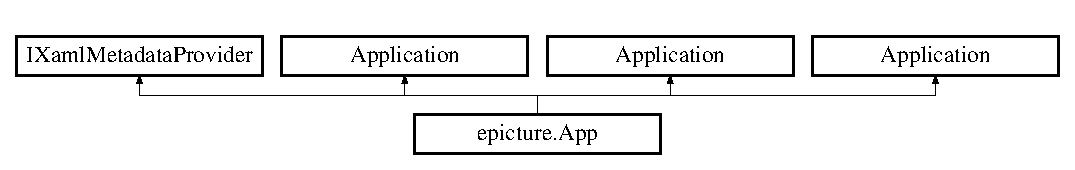
\includegraphics[height=1.842105cm]{classepicture_1_1_app}
\end{center}
\end{figure}
\subsection*{Public Member Functions}
\begin{DoxyCompactItemize}
\item 
\mbox{\hyperlink{classepicture_1_1_app_ac385b968cfe8c5cbb76009b068cd5009}{App}} ()
\begin{DoxyCompactList}\small\item\em Initialise l\textquotesingle{}objet d\textquotesingle{}application de singleton. Il s\textquotesingle{}agit de la première ligne du code créé à être exécutée. Elle correspond donc à l\textquotesingle{}équivalent logique de main() ou Win\+Main(). \end{DoxyCompactList}\item 
void \mbox{\hyperlink{classepicture_1_1_app_ab502a2fb60a201127ee980272694fa2c}{Initialize\+Component}} ()
\begin{DoxyCompactList}\small\item\em \mbox{\hyperlink{classepicture_1_1_app_ab502a2fb60a201127ee980272694fa2c}{Initialize\+Component()}} \end{DoxyCompactList}\item 
global\+::\+Windows.\+U\+I.\+Xaml.\+Markup.\+I\+Xaml\+Type \mbox{\hyperlink{classepicture_1_1_app_ad07aa9948de2fe3ccf94fc72747f6fe8}{Get\+Xaml\+Type}} (global\+::\+System.\+Type type)
\begin{DoxyCompactList}\small\item\em Get\+Xaml\+Type(\+Type) \end{DoxyCompactList}\item 
global\+::\+Windows.\+U\+I.\+Xaml.\+Markup.\+I\+Xaml\+Type \mbox{\hyperlink{classepicture_1_1_app_a5d41e2aede9485b8010a8c707be7d434}{Get\+Xaml\+Type}} (string full\+Name)
\begin{DoxyCompactList}\small\item\em Get\+Xaml\+Type(\+String) \end{DoxyCompactList}\item 
global\+::\+Windows.\+U\+I.\+Xaml.\+Markup.\+Xmlns\+Definition \mbox{[}$\,$\mbox{]} \mbox{\hyperlink{classepicture_1_1_app_a2e22f01b876b3511e2dbc9241ab1a2cc}{Get\+Xmlns\+Definitions}} ()
\begin{DoxyCompactList}\small\item\em \mbox{\hyperlink{classepicture_1_1_app_a2e22f01b876b3511e2dbc9241ab1a2cc}{Get\+Xmlns\+Definitions()}} \end{DoxyCompactList}\end{DoxyCompactItemize}
\subsection*{Protected Member Functions}
\begin{DoxyCompactItemize}
\item 
override void \mbox{\hyperlink{classepicture_1_1_app_a588834872f8c75103ef6b5ccb117e6fb}{On\+Launched}} (Launch\+Activated\+Event\+Args e)
\begin{DoxyCompactList}\small\item\em Invoqué lorsque l\textquotesingle{}application est lancée normalement par l\textquotesingle{}utilisateur final. D\textquotesingle{}autres points d\textquotesingle{}entrée seront utilisés par exemple au moment du lancement de l\textquotesingle{}application pour l\textquotesingle{}ouverture d\textquotesingle{}un fichier spécifique. \end{DoxyCompactList}\end{DoxyCompactItemize}
\subsection*{Private Member Functions}
\begin{DoxyCompactItemize}
\item 
void \mbox{\hyperlink{classepicture_1_1_app_a9878a4687b9b9dc2e7d24cd2501fd2c3}{On\+Navigation\+Failed}} (object sender, Navigation\+Failed\+Event\+Args e)
\begin{DoxyCompactList}\small\item\em Appelé lorsque la navigation vers une page donnée échoue \end{DoxyCompactList}\item 
void \mbox{\hyperlink{classepicture_1_1_app_afc42747b09fad5af9daba6e0121ced9a}{On\+Suspending}} (object sender, Suspending\+Event\+Args e)
\begin{DoxyCompactList}\small\item\em Appelé lorsque l\textquotesingle{}exécution de l\textquotesingle{}application est suspendue. L\textquotesingle{}état de l\textquotesingle{}application est enregistré sans savoir si l\textquotesingle{}application pourra se fermer ou reprendre sans endommager le contenu de la mémoire. \end{DoxyCompactList}\end{DoxyCompactItemize}
\subsection*{Private Attributes}
\begin{DoxyCompactItemize}
\item 
\mbox{\Hypertarget{classepicture_1_1_app_aef10db95121bd3a4a1c55676e8a522ad}\label{classepicture_1_1_app_aef10db95121bd3a4a1c55676e8a522ad}} 
bool {\bfseries \+\_\+content\+Loaded}
\item 
\mbox{\Hypertarget{classepicture_1_1_app_a8e79716acf270b1061eb1e47cb452044}\label{classepicture_1_1_app_a8e79716acf270b1061eb1e47cb452044}} 
global\+::epicture.\+epicture\+\_\+\+Xaml\+Type\+Info.\+Xaml\+Type\+Info\+Provider {\bfseries \+\_\+provider}
\end{DoxyCompactItemize}


\subsection{Detailed Description}
Fournit un comportement spécifique à l\textquotesingle{}application afin de compléter la classe Application par défaut. 



\subsection{Constructor \& Destructor Documentation}
\mbox{\Hypertarget{classepicture_1_1_app_ac385b968cfe8c5cbb76009b068cd5009}\label{classepicture_1_1_app_ac385b968cfe8c5cbb76009b068cd5009}} 
\index{epicture\+::\+App@{epicture\+::\+App}!App@{App}}
\index{App@{App}!epicture\+::\+App@{epicture\+::\+App}}
\subsubsection{\texorpdfstring{App()}{App()}}
{\footnotesize\ttfamily epicture.\+App.\+App (\begin{DoxyParamCaption}{ }\end{DoxyParamCaption})}



Initialise l\textquotesingle{}objet d\textquotesingle{}application de singleton. Il s\textquotesingle{}agit de la première ligne du code créé à être exécutée. Elle correspond donc à l\textquotesingle{}équivalent logique de main() ou Win\+Main(). 



\subsection{Member Function Documentation}
\mbox{\Hypertarget{classepicture_1_1_app_ad07aa9948de2fe3ccf94fc72747f6fe8}\label{classepicture_1_1_app_ad07aa9948de2fe3ccf94fc72747f6fe8}} 
\index{epicture\+::\+App@{epicture\+::\+App}!Get\+Xaml\+Type@{Get\+Xaml\+Type}}
\index{Get\+Xaml\+Type@{Get\+Xaml\+Type}!epicture\+::\+App@{epicture\+::\+App}}
\subsubsection{\texorpdfstring{Get\+Xaml\+Type()}{GetXamlType()}\hspace{0.1cm}{\footnotesize\ttfamily [1/2]}}
{\footnotesize\ttfamily global.\+Windows.\+U\+I.\+Xaml.\+Markup.\+I\+Xaml\+Type epicture.\+App.\+Get\+Xaml\+Type (\begin{DoxyParamCaption}\item[{global\+::\+System.\+Type}]{type }\end{DoxyParamCaption})}



Get\+Xaml\+Type(\+Type) 

\mbox{\Hypertarget{classepicture_1_1_app_a5d41e2aede9485b8010a8c707be7d434}\label{classepicture_1_1_app_a5d41e2aede9485b8010a8c707be7d434}} 
\index{epicture\+::\+App@{epicture\+::\+App}!Get\+Xaml\+Type@{Get\+Xaml\+Type}}
\index{Get\+Xaml\+Type@{Get\+Xaml\+Type}!epicture\+::\+App@{epicture\+::\+App}}
\subsubsection{\texorpdfstring{Get\+Xaml\+Type()}{GetXamlType()}\hspace{0.1cm}{\footnotesize\ttfamily [2/2]}}
{\footnotesize\ttfamily global.\+Windows.\+U\+I.\+Xaml.\+Markup.\+I\+Xaml\+Type epicture.\+App.\+Get\+Xaml\+Type (\begin{DoxyParamCaption}\item[{string}]{full\+Name }\end{DoxyParamCaption})}



Get\+Xaml\+Type(\+String) 

\mbox{\Hypertarget{classepicture_1_1_app_a2e22f01b876b3511e2dbc9241ab1a2cc}\label{classepicture_1_1_app_a2e22f01b876b3511e2dbc9241ab1a2cc}} 
\index{epicture\+::\+App@{epicture\+::\+App}!Get\+Xmlns\+Definitions@{Get\+Xmlns\+Definitions}}
\index{Get\+Xmlns\+Definitions@{Get\+Xmlns\+Definitions}!epicture\+::\+App@{epicture\+::\+App}}
\subsubsection{\texorpdfstring{Get\+Xmlns\+Definitions()}{GetXmlnsDefinitions()}}
{\footnotesize\ttfamily global.\+Windows.\+U\+I.\+Xaml.\+Markup.\+Xmlns\+Definition \mbox{[}$\,$\mbox{]} epicture.\+App.\+Get\+Xmlns\+Definitions (\begin{DoxyParamCaption}{ }\end{DoxyParamCaption})}



\mbox{\hyperlink{classepicture_1_1_app_a2e22f01b876b3511e2dbc9241ab1a2cc}{Get\+Xmlns\+Definitions()}} 

\mbox{\Hypertarget{classepicture_1_1_app_ab502a2fb60a201127ee980272694fa2c}\label{classepicture_1_1_app_ab502a2fb60a201127ee980272694fa2c}} 
\index{epicture\+::\+App@{epicture\+::\+App}!Initialize\+Component@{Initialize\+Component}}
\index{Initialize\+Component@{Initialize\+Component}!epicture\+::\+App@{epicture\+::\+App}}
\subsubsection{\texorpdfstring{Initialize\+Component()}{InitializeComponent()}}
{\footnotesize\ttfamily void epicture.\+App.\+Initialize\+Component (\begin{DoxyParamCaption}{ }\end{DoxyParamCaption})}



\mbox{\hyperlink{classepicture_1_1_app_ab502a2fb60a201127ee980272694fa2c}{Initialize\+Component()}} 

\mbox{\Hypertarget{classepicture_1_1_app_a588834872f8c75103ef6b5ccb117e6fb}\label{classepicture_1_1_app_a588834872f8c75103ef6b5ccb117e6fb}} 
\index{epicture\+::\+App@{epicture\+::\+App}!On\+Launched@{On\+Launched}}
\index{On\+Launched@{On\+Launched}!epicture\+::\+App@{epicture\+::\+App}}
\subsubsection{\texorpdfstring{On\+Launched()}{OnLaunched()}}
{\footnotesize\ttfamily override void epicture.\+App.\+On\+Launched (\begin{DoxyParamCaption}\item[{Launch\+Activated\+Event\+Args}]{e }\end{DoxyParamCaption})\hspace{0.3cm}{\ttfamily [protected]}}



Invoqué lorsque l\textquotesingle{}application est lancée normalement par l\textquotesingle{}utilisateur final. D\textquotesingle{}autres points d\textquotesingle{}entrée seront utilisés par exemple au moment du lancement de l\textquotesingle{}application pour l\textquotesingle{}ouverture d\textquotesingle{}un fichier spécifique. 


\begin{DoxyParams}{Parameters}
{\em e} & Détails concernant la requête et le processus de lancement.\\
\hline
\end{DoxyParams}
\mbox{\Hypertarget{classepicture_1_1_app_a9878a4687b9b9dc2e7d24cd2501fd2c3}\label{classepicture_1_1_app_a9878a4687b9b9dc2e7d24cd2501fd2c3}} 
\index{epicture\+::\+App@{epicture\+::\+App}!On\+Navigation\+Failed@{On\+Navigation\+Failed}}
\index{On\+Navigation\+Failed@{On\+Navigation\+Failed}!epicture\+::\+App@{epicture\+::\+App}}
\subsubsection{\texorpdfstring{On\+Navigation\+Failed()}{OnNavigationFailed()}}
{\footnotesize\ttfamily void epicture.\+App.\+On\+Navigation\+Failed (\begin{DoxyParamCaption}\item[{object}]{sender,  }\item[{Navigation\+Failed\+Event\+Args}]{e }\end{DoxyParamCaption})\hspace{0.3cm}{\ttfamily [private]}}



Appelé lorsque la navigation vers une page donnée échoue 


\begin{DoxyParams}{Parameters}
{\em sender} & Frame à l\textquotesingle{}origine de l\textquotesingle{}échec de navigation.\\
\hline
{\em e} & Détails relatifs à l\textquotesingle{}échec de navigation\\
\hline
\end{DoxyParams}
\mbox{\Hypertarget{classepicture_1_1_app_afc42747b09fad5af9daba6e0121ced9a}\label{classepicture_1_1_app_afc42747b09fad5af9daba6e0121ced9a}} 
\index{epicture\+::\+App@{epicture\+::\+App}!On\+Suspending@{On\+Suspending}}
\index{On\+Suspending@{On\+Suspending}!epicture\+::\+App@{epicture\+::\+App}}
\subsubsection{\texorpdfstring{On\+Suspending()}{OnSuspending()}}
{\footnotesize\ttfamily void epicture.\+App.\+On\+Suspending (\begin{DoxyParamCaption}\item[{object}]{sender,  }\item[{Suspending\+Event\+Args}]{e }\end{DoxyParamCaption})\hspace{0.3cm}{\ttfamily [private]}}



Appelé lorsque l\textquotesingle{}exécution de l\textquotesingle{}application est suspendue. L\textquotesingle{}état de l\textquotesingle{}application est enregistré sans savoir si l\textquotesingle{}application pourra se fermer ou reprendre sans endommager le contenu de la mémoire. 


\begin{DoxyParams}{Parameters}
{\em sender} & Source de la requête de suspension.\\
\hline
{\em e} & Détails de la requête de suspension.\\
\hline
\end{DoxyParams}


The documentation for this class was generated from the following files\+:\begin{DoxyCompactItemize}
\item 
epicture/epicture/App.\+xaml.\+cs\item 
epicture/epicture/obj/x86/\+Debug/App.\+g.\+i.\+cs\item 
epicture/epicture/obj/x86/\+Debug/Xaml\+Type\+Info.\+g.\+cs\end{DoxyCompactItemize}

\hypertarget{classepicture_test_1_1_app}{}\section{epicture\+Test.\+App Class Reference}
\label{classepicture_test_1_1_app}\index{epicture\+Test.\+App@{epicture\+Test.\+App}}


Provides application-\/specific behavior to supplement the default Application class.  


Inheritance diagram for epicture\+Test.\+App\+:\begin{figure}[H]
\begin{center}
\leavevmode
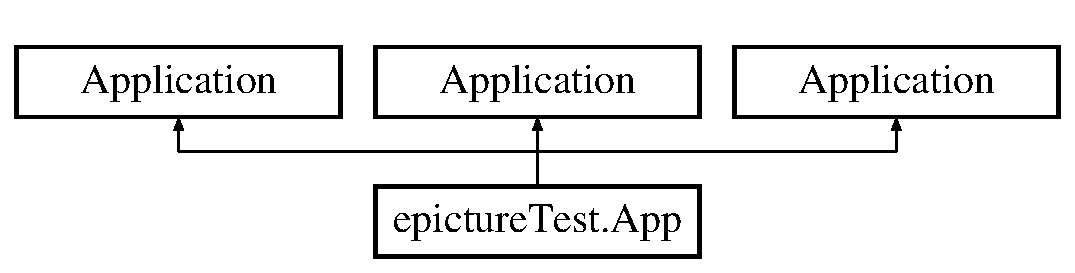
\includegraphics[height=2.000000cm]{classepicture_test_1_1_app}
\end{center}
\end{figure}
\subsection*{Public Member Functions}
\begin{DoxyCompactItemize}
\item 
void \mbox{\hyperlink{classepicture_test_1_1_app_aa0efa1442714a43751ba30d2adc7c61d}{Initialize\+Component}} ()
\begin{DoxyCompactList}\small\item\em \mbox{\hyperlink{classepicture_test_1_1_app_aa0efa1442714a43751ba30d2adc7c61d}{Initialize\+Component()}} \end{DoxyCompactList}\item 
\mbox{\hyperlink{classepicture_test_1_1_app_a66466105413d6f032cc51d14e38b8248}{App}} ()
\begin{DoxyCompactList}\small\item\em Initializes the singleton application object. This is the first line of authored code executed, and as such is the logical equivalent of main() or Win\+Main(). \end{DoxyCompactList}\end{DoxyCompactItemize}
\subsection*{Protected Member Functions}
\begin{DoxyCompactItemize}
\item 
override void \mbox{\hyperlink{classepicture_test_1_1_app_a2a8b2cc6742804e2107661d14e9f6f43}{On\+Launched}} (Launch\+Activated\+Event\+Args e)
\begin{DoxyCompactList}\small\item\em Invoked when the application is launched normally by the end user. Other entry points will be used such as when the application is launched to open a specific file. \end{DoxyCompactList}\end{DoxyCompactItemize}
\subsection*{Private Member Functions}
\begin{DoxyCompactItemize}
\item 
void \mbox{\hyperlink{classepicture_test_1_1_app_adec3d812ca9ceee7eff2ad6b9684fe7f}{On\+Navigation\+Failed}} (object sender, Navigation\+Failed\+Event\+Args e)
\begin{DoxyCompactList}\small\item\em Invoked when Navigation to a certain page fails \end{DoxyCompactList}\item 
void \mbox{\hyperlink{classepicture_test_1_1_app_afd75e91ae3342f538aedc20e398f8f4a}{On\+Suspending}} (object sender, Suspending\+Event\+Args e)
\begin{DoxyCompactList}\small\item\em Invoked when application execution is being suspended. Application state is saved without knowing whether the application will be terminated or resumed with the contents of memory still intact. \end{DoxyCompactList}\end{DoxyCompactItemize}
\subsection*{Private Attributes}
\begin{DoxyCompactItemize}
\item 
\mbox{\Hypertarget{classepicture_test_1_1_app_af0124bfdcd32ce132d304217c798cc76}\label{classepicture_test_1_1_app_af0124bfdcd32ce132d304217c798cc76}} 
bool {\bfseries \+\_\+content\+Loaded}
\end{DoxyCompactItemize}


\subsection{Detailed Description}
Provides application-\/specific behavior to supplement the default Application class. 



\subsection{Constructor \& Destructor Documentation}
\mbox{\Hypertarget{classepicture_test_1_1_app_a66466105413d6f032cc51d14e38b8248}\label{classepicture_test_1_1_app_a66466105413d6f032cc51d14e38b8248}} 
\index{epicture\+Test\+::\+App@{epicture\+Test\+::\+App}!App@{App}}
\index{App@{App}!epicture\+Test\+::\+App@{epicture\+Test\+::\+App}}
\subsubsection{\texorpdfstring{App()}{App()}}
{\footnotesize\ttfamily epicture\+Test.\+App.\+App (\begin{DoxyParamCaption}{ }\end{DoxyParamCaption})}



Initializes the singleton application object. This is the first line of authored code executed, and as such is the logical equivalent of main() or Win\+Main(). 



\subsection{Member Function Documentation}
\mbox{\Hypertarget{classepicture_test_1_1_app_aa0efa1442714a43751ba30d2adc7c61d}\label{classepicture_test_1_1_app_aa0efa1442714a43751ba30d2adc7c61d}} 
\index{epicture\+Test\+::\+App@{epicture\+Test\+::\+App}!Initialize\+Component@{Initialize\+Component}}
\index{Initialize\+Component@{Initialize\+Component}!epicture\+Test\+::\+App@{epicture\+Test\+::\+App}}
\subsubsection{\texorpdfstring{Initialize\+Component()}{InitializeComponent()}}
{\footnotesize\ttfamily void epicture\+Test.\+App.\+Initialize\+Component (\begin{DoxyParamCaption}{ }\end{DoxyParamCaption})}



\mbox{\hyperlink{classepicture_test_1_1_app_aa0efa1442714a43751ba30d2adc7c61d}{Initialize\+Component()}} 

\mbox{\Hypertarget{classepicture_test_1_1_app_a2a8b2cc6742804e2107661d14e9f6f43}\label{classepicture_test_1_1_app_a2a8b2cc6742804e2107661d14e9f6f43}} 
\index{epicture\+Test\+::\+App@{epicture\+Test\+::\+App}!On\+Launched@{On\+Launched}}
\index{On\+Launched@{On\+Launched}!epicture\+Test\+::\+App@{epicture\+Test\+::\+App}}
\subsubsection{\texorpdfstring{On\+Launched()}{OnLaunched()}}
{\footnotesize\ttfamily override void epicture\+Test.\+App.\+On\+Launched (\begin{DoxyParamCaption}\item[{Launch\+Activated\+Event\+Args}]{e }\end{DoxyParamCaption})\hspace{0.3cm}{\ttfamily [protected]}}



Invoked when the application is launched normally by the end user. Other entry points will be used such as when the application is launched to open a specific file. 


\begin{DoxyParams}{Parameters}
{\em e} & Details about the launch request and process.\\
\hline
\end{DoxyParams}
\mbox{\Hypertarget{classepicture_test_1_1_app_adec3d812ca9ceee7eff2ad6b9684fe7f}\label{classepicture_test_1_1_app_adec3d812ca9ceee7eff2ad6b9684fe7f}} 
\index{epicture\+Test\+::\+App@{epicture\+Test\+::\+App}!On\+Navigation\+Failed@{On\+Navigation\+Failed}}
\index{On\+Navigation\+Failed@{On\+Navigation\+Failed}!epicture\+Test\+::\+App@{epicture\+Test\+::\+App}}
\subsubsection{\texorpdfstring{On\+Navigation\+Failed()}{OnNavigationFailed()}}
{\footnotesize\ttfamily void epicture\+Test.\+App.\+On\+Navigation\+Failed (\begin{DoxyParamCaption}\item[{object}]{sender,  }\item[{Navigation\+Failed\+Event\+Args}]{e }\end{DoxyParamCaption})\hspace{0.3cm}{\ttfamily [private]}}



Invoked when Navigation to a certain page fails 


\begin{DoxyParams}{Parameters}
{\em sender} & The Frame which failed navigation\\
\hline
{\em e} & Details about the navigation failure\\
\hline
\end{DoxyParams}
\mbox{\Hypertarget{classepicture_test_1_1_app_afd75e91ae3342f538aedc20e398f8f4a}\label{classepicture_test_1_1_app_afd75e91ae3342f538aedc20e398f8f4a}} 
\index{epicture\+Test\+::\+App@{epicture\+Test\+::\+App}!On\+Suspending@{On\+Suspending}}
\index{On\+Suspending@{On\+Suspending}!epicture\+Test\+::\+App@{epicture\+Test\+::\+App}}
\subsubsection{\texorpdfstring{On\+Suspending()}{OnSuspending()}}
{\footnotesize\ttfamily void epicture\+Test.\+App.\+On\+Suspending (\begin{DoxyParamCaption}\item[{object}]{sender,  }\item[{Suspending\+Event\+Args}]{e }\end{DoxyParamCaption})\hspace{0.3cm}{\ttfamily [private]}}



Invoked when application execution is being suspended. Application state is saved without knowing whether the application will be terminated or resumed with the contents of memory still intact. 


\begin{DoxyParams}{Parameters}
{\em sender} & The source of the suspend request.\\
\hline
{\em e} & Details about the suspend request.\\
\hline
\end{DoxyParams}


The documentation for this class was generated from the following files\+:\begin{DoxyCompactItemize}
\item 
epicture/epicture\+Test/obj/x86/\+Debug/Unit\+Test\+App.\+g.\+cs\item 
epicture/epicture\+Test/obj/x86/\+Debug/Unit\+Test\+App.\+g.\+i.\+cs\item 
epicture/epicture\+Test/Unit\+Test\+App.\+xaml.\+cs\end{DoxyCompactItemize}

\hypertarget{classepicture_1_1_flickr_api}{}\section{epicture.\+Flickr\+Api Class Reference}
\label{classepicture_1_1_flickr_api}\index{epicture.\+Flickr\+Api@{epicture.\+Flickr\+Api}}
\subsection*{Public Member Functions}
\begin{DoxyCompactItemize}
\item 
async Task$<$ \mbox{\hyperlink{classepicture_1_1_image_container}{Image\+Container}} $>$ \mbox{\hyperlink{classepicture_1_1_flickr_api_abd70a1f8fe82ddc219572058be51dd51}{create\+Image\+Container\+From\+Tag}} (string tag, int nb\+\_\+photos)
\item 
async void \mbox{\hyperlink{classepicture_1_1_flickr_api_a4e39f3d53b58577718284c284c34338b}{Test\+Login}} ()
\item 
async void \mbox{\hyperlink{classepicture_1_1_flickr_api_a148c12d8328b94be08a554a45a546fc1}{Oauth}} ()
\end{DoxyCompactItemize}
\subsection*{Static Public Member Functions}
\begin{DoxyCompactItemize}
\item 
\mbox{\Hypertarget{classepicture_1_1_flickr_api_a387ed0b89c15b93cce6722bda643b92f}\label{classepicture_1_1_flickr_api_a387ed0b89c15b93cce6722bda643b92f}} 
static Flickr {\bfseries Get\+Instance} ()
\end{DoxyCompactItemize}
\subsection*{Private Member Functions}
\begin{DoxyCompactItemize}
\item 
async Task$<$ string $>$ \mbox{\hyperlink{classepicture_1_1_flickr_api_ae914f2cefba1eb20021af69115471626}{Send\+Data\+Async}} (String Url)
\item 
String \mbox{\hyperlink{classepicture_1_1_flickr_api_a9ab15abcbe6c3002eb753dd79aa587ae}{Parse\+Token}} (String to\+Find, String response)
\item 
async void \mbox{\hyperlink{classepicture_1_1_flickr_api_af613a836598d8cdccde548b2b4d16c5c}{Exchange\+Request\+Token\+With\+Oauth\+Token}} (String Token\+Uri, String Token\+Secret\+Tmp)
\end{DoxyCompactItemize}
\subsection*{Private Attributes}
\begin{DoxyCompactItemize}
\item 
\mbox{\Hypertarget{classepicture_1_1_flickr_api_a6f1e1718b8dc79e8857f9ea71879fb75}\label{classepicture_1_1_flickr_api_a6f1e1718b8dc79e8857f9ea71879fb75}} 
const string {\bfseries A\+P\+I\+\_\+\+K\+EY} = \char`\"{}ed97463b02210fa18ccfe6a1358267b3\char`\"{}
\item 
\mbox{\Hypertarget{classepicture_1_1_flickr_api_a88b3b145ac8b7cfb264b992c215ccfde}\label{classepicture_1_1_flickr_api_a88b3b145ac8b7cfb264b992c215ccfde}} 
const string {\bfseries A\+P\+I\+\_\+\+S\+E\+C\+R\+ET} = \char`\"{}d6826b8008652f89\char`\"{}
\item 
const string \mbox{\hyperlink{classepicture_1_1_flickr_api_aa2d58a7bd6de20766896ad0b717100bb}{A\+P\+I\+\_\+\+C\+A\+L\+L\+B\+A\+CK}} = \char`\"{}ms-\/appx-\/web\+://Microsoft.\+A\+A\+D.\+Broker\+Plug\+In/S-\/1-\/15-\/2-\/660250367-\/210907714-\/264770912-\/2147469295-\/3070322386-\/383610947-\/1518229695\char`\"{}
\item 
\mbox{\Hypertarget{classepicture_1_1_flickr_api_a278659143c782dc0f3d0cd5af4f44513}\label{classepicture_1_1_flickr_api_a278659143c782dc0f3d0cd5af4f44513}} 
String {\bfseries Secret\+Token}
\item 
\mbox{\Hypertarget{classepicture_1_1_flickr_api_a0ca06cbf2214c4ba041803f7eafa3317}\label{classepicture_1_1_flickr_api_a0ca06cbf2214c4ba041803f7eafa3317}} 
String {\bfseries Access\+Token}
\item 
\mbox{\Hypertarget{classepicture_1_1_flickr_api_a241660e21ea428b33ff3c6157eeb3ed9}\label{classepicture_1_1_flickr_api_a241660e21ea428b33ff3c6157eeb3ed9}} 
Flickr {\bfseries flickr}
\item 
\mbox{\Hypertarget{classepicture_1_1_flickr_api_a2ab99ed8b12c50cd07de3bec64eadc74}\label{classepicture_1_1_flickr_api_a2ab99ed8b12c50cd07de3bec64eadc74}} 
\mbox{\hyperlink{classepicture_1_1_helper}{Helper}} {\bfseries Helper}
\end{DoxyCompactItemize}


\subsection{Detailed Description}
Flickr\+A\+PI will allow us to interact with Flickr and get pictures and so on... 

\subsection{Member Function Documentation}
\mbox{\Hypertarget{classepicture_1_1_flickr_api_abd70a1f8fe82ddc219572058be51dd51}\label{classepicture_1_1_flickr_api_abd70a1f8fe82ddc219572058be51dd51}} 
\index{epicture\+::\+Flickr\+Api@{epicture\+::\+Flickr\+Api}!create\+Image\+Container\+From\+Tag@{create\+Image\+Container\+From\+Tag}}
\index{create\+Image\+Container\+From\+Tag@{create\+Image\+Container\+From\+Tag}!epicture\+::\+Flickr\+Api@{epicture\+::\+Flickr\+Api}}
\subsubsection{\texorpdfstring{create\+Image\+Container\+From\+Tag()}{createImageContainerFromTag()}}
{\footnotesize\ttfamily async Task$<$\mbox{\hyperlink{classepicture_1_1_image_container}{Image\+Container}}$>$ epicture.\+Flickr\+Api.\+create\+Image\+Container\+From\+Tag (\begin{DoxyParamCaption}\item[{string}]{tag,  }\item[{int}]{nb\+\_\+photos }\end{DoxyParamCaption})}

This method extract images with a certain tag 
\begin{DoxyParams}{Parameters}
{\em tag} & the tag\textquotesingle{}s name \\
\hline
{\em nb\+\_\+photos} & the number of pictures. \\
\hline
\end{DoxyParams}
\mbox{\Hypertarget{classepicture_1_1_flickr_api_af613a836598d8cdccde548b2b4d16c5c}\label{classepicture_1_1_flickr_api_af613a836598d8cdccde548b2b4d16c5c}} 
\index{epicture\+::\+Flickr\+Api@{epicture\+::\+Flickr\+Api}!Exchange\+Request\+Token\+With\+Oauth\+Token@{Exchange\+Request\+Token\+With\+Oauth\+Token}}
\index{Exchange\+Request\+Token\+With\+Oauth\+Token@{Exchange\+Request\+Token\+With\+Oauth\+Token}!epicture\+::\+Flickr\+Api@{epicture\+::\+Flickr\+Api}}
\subsubsection{\texorpdfstring{Exchange\+Request\+Token\+With\+Oauth\+Token()}{ExchangeRequestTokenWithOauthToken()}}
{\footnotesize\ttfamily async void epicture.\+Flickr\+Api.\+Exchange\+Request\+Token\+With\+Oauth\+Token (\begin{DoxyParamCaption}\item[{String}]{Token\+Uri,  }\item[{String}]{Token\+Secret\+Tmp }\end{DoxyParamCaption})\hspace{0.3cm}{\ttfamily [private]}}

Exchange the request token for the access token 
\begin{DoxyParams}{Parameters}
{\em Token\+Uri} & Token Uri wich is the response of the O\+Auth Request Query \\
\hline
{\em Token\+Secret\+Tmp} & Secret Token obtained by Request Token Query \\
\hline
\end{DoxyParams}
\mbox{\Hypertarget{classepicture_1_1_flickr_api_a148c12d8328b94be08a554a45a546fc1}\label{classepicture_1_1_flickr_api_a148c12d8328b94be08a554a45a546fc1}} 
\index{epicture\+::\+Flickr\+Api@{epicture\+::\+Flickr\+Api}!Oauth@{Oauth}}
\index{Oauth@{Oauth}!epicture\+::\+Flickr\+Api@{epicture\+::\+Flickr\+Api}}
\subsubsection{\texorpdfstring{Oauth()}{Oauth()}}
{\footnotesize\ttfamily async void epicture.\+Flickr\+Api.\+Oauth (\begin{DoxyParamCaption}{ }\end{DoxyParamCaption})}

Main authentication function \mbox{\Hypertarget{classepicture_1_1_flickr_api_a9ab15abcbe6c3002eb753dd79aa587ae}\label{classepicture_1_1_flickr_api_a9ab15abcbe6c3002eb753dd79aa587ae}} 
\index{epicture\+::\+Flickr\+Api@{epicture\+::\+Flickr\+Api}!Parse\+Token@{Parse\+Token}}
\index{Parse\+Token@{Parse\+Token}!epicture\+::\+Flickr\+Api@{epicture\+::\+Flickr\+Api}}
\subsubsection{\texorpdfstring{Parse\+Token()}{ParseToken()}}
{\footnotesize\ttfamily String epicture.\+Flickr\+Api.\+Parse\+Token (\begin{DoxyParamCaption}\item[{String}]{to\+Find,  }\item[{String}]{response }\end{DoxyParamCaption})\hspace{0.3cm}{\ttfamily [private]}}

This method extract the value from the Token 
\begin{DoxyParams}{Parameters}
{\em to\+Find} & Pattern to find \\
\hline
{\em response} & String to parse \\
\hline
\end{DoxyParams}
\mbox{\Hypertarget{classepicture_1_1_flickr_api_ae914f2cefba1eb20021af69115471626}\label{classepicture_1_1_flickr_api_ae914f2cefba1eb20021af69115471626}} 
\index{epicture\+::\+Flickr\+Api@{epicture\+::\+Flickr\+Api}!Send\+Data\+Async@{Send\+Data\+Async}}
\index{Send\+Data\+Async@{Send\+Data\+Async}!epicture\+::\+Flickr\+Api@{epicture\+::\+Flickr\+Api}}
\subsubsection{\texorpdfstring{Send\+Data\+Async()}{SendDataAsync()}}
{\footnotesize\ttfamily async Task$<$string$>$ epicture.\+Flickr\+Api.\+Send\+Data\+Async (\begin{DoxyParamCaption}\item[{String}]{Url }\end{DoxyParamCaption})\hspace{0.3cm}{\ttfamily [private]}}

This method execute a asyncronous H\+T\+TP Request 
\begin{DoxyParams}{Parameters}
{\em Url} & url to request \\
\hline
\end{DoxyParams}
\mbox{\Hypertarget{classepicture_1_1_flickr_api_a4e39f3d53b58577718284c284c34338b}\label{classepicture_1_1_flickr_api_a4e39f3d53b58577718284c284c34338b}} 
\index{epicture\+::\+Flickr\+Api@{epicture\+::\+Flickr\+Api}!Test\+Login@{Test\+Login}}
\index{Test\+Login@{Test\+Login}!epicture\+::\+Flickr\+Api@{epicture\+::\+Flickr\+Api}}
\subsubsection{\texorpdfstring{Test\+Login()}{TestLogin()}}
{\footnotesize\ttfamily async void epicture.\+Flickr\+Api.\+Test\+Login (\begin{DoxyParamCaption}{ }\end{DoxyParamCaption})}

this method is a test from the authentication 

\subsection{Member Data Documentation}
\mbox{\Hypertarget{classepicture_1_1_flickr_api_aa2d58a7bd6de20766896ad0b717100bb}\label{classepicture_1_1_flickr_api_aa2d58a7bd6de20766896ad0b717100bb}} 
\index{epicture\+::\+Flickr\+Api@{epicture\+::\+Flickr\+Api}!A\+P\+I\+\_\+\+C\+A\+L\+L\+B\+A\+CK@{A\+P\+I\+\_\+\+C\+A\+L\+L\+B\+A\+CK}}
\index{A\+P\+I\+\_\+\+C\+A\+L\+L\+B\+A\+CK@{A\+P\+I\+\_\+\+C\+A\+L\+L\+B\+A\+CK}!epicture\+::\+Flickr\+Api@{epicture\+::\+Flickr\+Api}}
\subsubsection{\texorpdfstring{A\+P\+I\+\_\+\+C\+A\+L\+L\+B\+A\+CK}{API\_CALLBACK}}
{\footnotesize\ttfamily const string epicture.\+Flickr\+Api.\+A\+P\+I\+\_\+\+C\+A\+L\+L\+B\+A\+CK = \char`\"{}ms-\/appx-\/web\+://Microsoft.\+A\+A\+D.\+Broker\+Plug\+In/S-\/1-\/15-\/2-\/660250367-\/210907714-\/264770912-\/2147469295-\/3070322386-\/383610947-\/1518229695\char`\"{}\hspace{0.3cm}{\ttfamily [private]}}

The callback U\+RL to redirect the user back to the program 

The documentation for this class was generated from the following file\+:\begin{DoxyCompactItemize}
\item 
epicture/epicture\+Library/Flickr\+Api.\+cs\end{DoxyCompactItemize}

\hypertarget{classepicture_1_1_helper}{}\section{epicture.\+Helper Class Reference}
\label{classepicture_1_1_helper}\index{epicture.\+Helper@{epicture.\+Helper}}
\subsection*{Public Member Functions}
\begin{DoxyCompactItemize}
\item 
\mbox{\Hypertarget{classepicture_1_1_helper_a97c8f872400d13dcf35f79d07c5d6c18}\label{classepicture_1_1_helper_a97c8f872400d13dcf35f79d07c5d6c18}} 
{\bfseries Helper} (String \+\_\+api\+Key, String \+\_\+api\+Secret, String \+\_\+api\+Callback)
\item 
String \mbox{\hyperlink{classepicture_1_1_helper_a82fe7fbebbb5cee5e7787d5f7062bb5f}{Query\+Get\+Access\+Token}} (String secret\+Token\+Tmp, String oauth\+Token, String oauth\+Verifier)
\item 
String \mbox{\hyperlink{classepicture_1_1_helper_a9a42fa4d53acaed05f4985c8b2804417}{Query\+Get\+Oauth\+Url}} (String secret\+Token)
\item 
String \mbox{\hyperlink{classepicture_1_1_helper_ab01acef7d30c0270753f5deb838b993e}{Query\+Test\+Login}} (String access\+Token, String secret\+Token)
\item 
async Task$<$ Web\+Authentication\+Result $>$ \mbox{\hyperlink{classepicture_1_1_helper_af18b551f1629ecc0e6d8cacf1e9a4770}{Authenticate\+User}} (String oauth\+Token)
\item 
String \mbox{\hyperlink{classepicture_1_1_helper_a4ef537048b54f85c7f3e1a4c400e0b10}{Sign\+Me\+That}} (String Sig\+Base\+String, String token\+Secret)
\end{DoxyCompactItemize}
\subsection*{Private Attributes}
\begin{DoxyCompactItemize}
\item 
\mbox{\Hypertarget{classepicture_1_1_helper_ac8fe9d1a7744bff69020ed3b1f654490}\label{classepicture_1_1_helper_ac8fe9d1a7744bff69020ed3b1f654490}} 
String {\bfseries A\+P\+I\+\_\+\+K\+EY}
\item 
\mbox{\Hypertarget{classepicture_1_1_helper_a9ba3a50bd3aed5c6b420bcda4a8b8d60}\label{classepicture_1_1_helper_a9ba3a50bd3aed5c6b420bcda4a8b8d60}} 
String {\bfseries A\+P\+I\+\_\+\+S\+E\+C\+R\+ET}
\item 
\mbox{\Hypertarget{classepicture_1_1_helper_acb2a04675547389a46a2b5877b7eefb7}\label{classepicture_1_1_helper_acb2a04675547389a46a2b5877b7eefb7}} 
String {\bfseries A\+P\+I\+\_\+\+C\+A\+L\+L\+B\+A\+CK}
\end{DoxyCompactItemize}


\subsection{Member Function Documentation}
\mbox{\Hypertarget{classepicture_1_1_helper_af18b551f1629ecc0e6d8cacf1e9a4770}\label{classepicture_1_1_helper_af18b551f1629ecc0e6d8cacf1e9a4770}} 
\index{epicture\+::\+Helper@{epicture\+::\+Helper}!Authenticate\+User@{Authenticate\+User}}
\index{Authenticate\+User@{Authenticate\+User}!epicture\+::\+Helper@{epicture\+::\+Helper}}
\subsubsection{\texorpdfstring{Authenticate\+User()}{AuthenticateUser()}}
{\footnotesize\ttfamily async Task$<$Web\+Authentication\+Result$>$ epicture.\+Helper.\+Authenticate\+User (\begin{DoxyParamCaption}\item[{String}]{oauth\+Token }\end{DoxyParamCaption})}

Web Broker Windows to Authenticate the User with Oauth1 Technology \mbox{\Hypertarget{classepicture_1_1_helper_a82fe7fbebbb5cee5e7787d5f7062bb5f}\label{classepicture_1_1_helper_a82fe7fbebbb5cee5e7787d5f7062bb5f}} 
\index{epicture\+::\+Helper@{epicture\+::\+Helper}!Query\+Get\+Access\+Token@{Query\+Get\+Access\+Token}}
\index{Query\+Get\+Access\+Token@{Query\+Get\+Access\+Token}!epicture\+::\+Helper@{epicture\+::\+Helper}}
\subsubsection{\texorpdfstring{Query\+Get\+Access\+Token()}{QueryGetAccessToken()}}
{\footnotesize\ttfamily String epicture.\+Helper.\+Query\+Get\+Access\+Token (\begin{DoxyParamCaption}\item[{String}]{secret\+Token\+Tmp,  }\item[{String}]{oauth\+Token,  }\item[{String}]{oauth\+Verifier }\end{DoxyParamCaption})}

Query to get the access token thanks to secret\+Token and token verifier \mbox{\Hypertarget{classepicture_1_1_helper_a9a42fa4d53acaed05f4985c8b2804417}\label{classepicture_1_1_helper_a9a42fa4d53acaed05f4985c8b2804417}} 
\index{epicture\+::\+Helper@{epicture\+::\+Helper}!Query\+Get\+Oauth\+Url@{Query\+Get\+Oauth\+Url}}
\index{Query\+Get\+Oauth\+Url@{Query\+Get\+Oauth\+Url}!epicture\+::\+Helper@{epicture\+::\+Helper}}
\subsubsection{\texorpdfstring{Query\+Get\+Oauth\+Url()}{QueryGetOauthUrl()}}
{\footnotesize\ttfamily String epicture.\+Helper.\+Query\+Get\+Oauth\+Url (\begin{DoxyParamCaption}\item[{String}]{secret\+Token }\end{DoxyParamCaption})}

Query to get the Request token and the token verifier. \mbox{\Hypertarget{classepicture_1_1_helper_ab01acef7d30c0270753f5deb838b993e}\label{classepicture_1_1_helper_ab01acef7d30c0270753f5deb838b993e}} 
\index{epicture\+::\+Helper@{epicture\+::\+Helper}!Query\+Test\+Login@{Query\+Test\+Login}}
\index{Query\+Test\+Login@{Query\+Test\+Login}!epicture\+::\+Helper@{epicture\+::\+Helper}}
\subsubsection{\texorpdfstring{Query\+Test\+Login()}{QueryTestLogin()}}
{\footnotesize\ttfamily String epicture.\+Helper.\+Query\+Test\+Login (\begin{DoxyParamCaption}\item[{String}]{access\+Token,  }\item[{String}]{secret\+Token }\end{DoxyParamCaption})}

Request to test the Authentification. \mbox{\Hypertarget{classepicture_1_1_helper_a4ef537048b54f85c7f3e1a4c400e0b10}\label{classepicture_1_1_helper_a4ef537048b54f85c7f3e1a4c400e0b10}} 
\index{epicture\+::\+Helper@{epicture\+::\+Helper}!Sign\+Me\+That@{Sign\+Me\+That}}
\index{Sign\+Me\+That@{Sign\+Me\+That}!epicture\+::\+Helper@{epicture\+::\+Helper}}
\subsubsection{\texorpdfstring{Sign\+Me\+That()}{SignMeThat()}}
{\footnotesize\ttfamily String epicture.\+Helper.\+Sign\+Me\+That (\begin{DoxyParamCaption}\item[{String}]{Sig\+Base\+String,  }\item[{String}]{token\+Secret }\end{DoxyParamCaption})}

Signature of Request to be authorized of doing Request 
\begin{DoxyParams}{Parameters}
{\em Sig\+Base\+String} & U\+RL To Sign \\
\hline
{\em token\+Secret} & Token Secret to Sign \\
\hline
\end{DoxyParams}


The documentation for this class was generated from the following file\+:\begin{DoxyCompactItemize}
\item 
epicture/epicture\+Library/Helper.\+cs\end{DoxyCompactItemize}

\hypertarget{classepicture_1_1_image_container}{}\section{epicture.\+Image\+Container Class Reference}
\label{classepicture_1_1_image_container}\index{epicture.\+Image\+Container@{epicture.\+Image\+Container}}
\subsection*{Public Member Functions}
\begin{DoxyCompactItemize}
\item 
\mbox{\Hypertarget{classepicture_1_1_image_container_aeefd3ffbd166c933ce02b55fa21f842b}\label{classepicture_1_1_image_container_aeefd3ffbd166c933ce02b55fa21f842b}} 
void {\bfseries Add\+Image\+Source} (Image img)
\item 
\mbox{\Hypertarget{classepicture_1_1_image_container_ad34fd9cb915da8085bde614fcb3853c4}\label{classepicture_1_1_image_container_ad34fd9cb915da8085bde614fcb3853c4}} 
List$<$ Image $>$ {\bfseries Get\+Images} ()
\item 
\mbox{\Hypertarget{classepicture_1_1_image_container_aca03c1fe0000f454a1b3da6557b8a65c}\label{classepicture_1_1_image_container_aca03c1fe0000f454a1b3da6557b8a65c}} 
int {\bfseries Get\+Nb\+Images} ()
\end{DoxyCompactItemize}
\subsection*{Private Attributes}
\begin{DoxyCompactItemize}
\item 
\mbox{\Hypertarget{classepicture_1_1_image_container_ad2c3200320969e816372986b007b70ff}\label{classepicture_1_1_image_container_ad2c3200320969e816372986b007b70ff}} 
List$<$ Image $>$ {\bfseries \+\_\+images} = new List$<$Image$>$()
\end{DoxyCompactItemize}


The documentation for this class was generated from the following file\+:\begin{DoxyCompactItemize}
\item 
epicture/epicture\+Library/Image\+Container.\+cs\end{DoxyCompactItemize}

\hypertarget{classepicture_test_1_1_image_container_test}{}\section{epicture\+Test.\+Image\+Container\+Test Class Reference}
\label{classepicture_test_1_1_image_container_test}\index{epicture\+Test.\+Image\+Container\+Test@{epicture\+Test.\+Image\+Container\+Test}}
\subsection*{Public Member Functions}
\begin{DoxyCompactItemize}
\item 
\mbox{\Hypertarget{classepicture_test_1_1_image_container_test_ae98f92baeb2a6b5b6a00ec4d391574b7}\label{classepicture_test_1_1_image_container_test_ae98f92baeb2a6b5b6a00ec4d391574b7}} 
void {\bfseries empty\+List\+Test} ()
\item 
\mbox{\Hypertarget{classepicture_test_1_1_image_container_test_ac4bc137644c112217b02114a7088763c}\label{classepicture_test_1_1_image_container_test_ac4bc137644c112217b02114a7088763c}} 
void {\bfseries five\+Items\+List\+Test} ()
\end{DoxyCompactItemize}


The documentation for this class was generated from the following file\+:\begin{DoxyCompactItemize}
\item 
epicture/epicture\+Test/Image\+Container\+Test.\+cs\end{DoxyCompactItemize}

\hypertarget{classepicture_1_1_imgur_api}{}\section{epicture.\+Imgur\+Api Class Reference}
\label{classepicture_1_1_imgur_api}\index{epicture.\+Imgur\+Api@{epicture.\+Imgur\+Api}}
\subsection*{Public Member Functions}
\begin{DoxyCompactItemize}
\item 
\mbox{\Hypertarget{classepicture_1_1_imgur_api_a7d14cc12e95904ccb278443ce30d70b9}\label{classepicture_1_1_imgur_api_a7d14cc12e95904ccb278443ce30d70b9}} 
string {\bfseries get\+Access\+Token} ()
\item 
\mbox{\Hypertarget{classepicture_1_1_imgur_api_a4e6484b3040b1519dc6bbc721e2e074f}\label{classepicture_1_1_imgur_api_a4e6484b3040b1519dc6bbc721e2e074f}} 
void {\bfseries set\+Access\+Token} (string access\+\_\+token)
\item 
\mbox{\Hypertarget{classepicture_1_1_imgur_api_ad8ebbd689e638e24f11cd763658640fe}\label{classepicture_1_1_imgur_api_ad8ebbd689e638e24f11cd763658640fe}} 
async void {\bfseries get\+Token} ()
\item 
async Task$<$ String $>$ \mbox{\hyperlink{classepicture_1_1_imgur_api_a3ddaf3c09b2d5edf39ace0f2390f78a9}{call\+Back\+U\+RL}} ()
\item 
\mbox{\Hypertarget{classepicture_1_1_imgur_api_aebdd7484625ef704946e3966933db563}\label{classepicture_1_1_imgur_api_aebdd7484625ef704946e3966933db563}} 
async void {\bfseries add\+Favorites} (string id)
\item 
\mbox{\Hypertarget{classepicture_1_1_imgur_api_af0cb0b13ba443097dbde0980267b9b20}\label{classepicture_1_1_imgur_api_af0cb0b13ba443097dbde0980267b9b20}} 
async Task$<$ String $>$ {\bfseries connection} ()
\item 
\mbox{\Hypertarget{classepicture_1_1_imgur_api_affe36b9f3403dfbfdfbdea7811c54453}\label{classepicture_1_1_imgur_api_affe36b9f3403dfbfdfbdea7811c54453}} 
bool {\bfseries is\+Connected} ()
\item 
async Task$<$ \mbox{\hyperlink{classepicture_1_1_image_container}{Image\+Container}} $>$ \mbox{\hyperlink{classepicture_1_1_imgur_api_ac4db02936c30dfc87f1b5557f7a7af75}{create\+Image\+Container\+From\+Tag}} (string tag, int nb\+\_\+photos)
\item 
async Task$<$ \mbox{\hyperlink{classepicture_1_1_image_container}{Image\+Container}} $>$ \mbox{\hyperlink{classepicture_1_1_imgur_api_a105393adc1ac69c9be3fbd9c020c1b57}{create\+Image\+Container\+From\+Favorites}} ()
\item 
async Task$<$ \mbox{\hyperlink{classepicture_1_1_image_container}{Image\+Container}} $>$ \mbox{\hyperlink{classepicture_1_1_imgur_api_a7d7e217e9bbe707827de3f3222245ba8}{create\+Image\+Container\+From\+Posts}} ()
\item 
async void \mbox{\hyperlink{classepicture_1_1_imgur_api_a9f5cec5e327a823db214ff4d4738197a}{post\+Image}} (string filename)
\item 
\mbox{\Hypertarget{classepicture_1_1_imgur_api_aeb84a9fc83ef5d634a9196654384eb5b}\label{classepicture_1_1_imgur_api_aeb84a9fc83ef5d634a9196654384eb5b}} 
async void {\bfseries delete\+Post} (string id)
\end{DoxyCompactItemize}
\subsection*{Private Attributes}
\begin{DoxyCompactItemize}
\item 
\mbox{\Hypertarget{classepicture_1_1_imgur_api_abef6924a5498e830d010efeb123f6f47}\label{classepicture_1_1_imgur_api_abef6924a5498e830d010efeb123f6f47}} 
Image\+Endpoint {\bfseries endpoint}
\item 
\mbox{\Hypertarget{classepicture_1_1_imgur_api_a586a3f3f53f1756ae50c9e93510a8bce}\label{classepicture_1_1_imgur_api_a586a3f3f53f1756ae50c9e93510a8bce}} 
string {\bfseries client\+\_\+id} = \char`\"{}48a61c1ae13d63e\char`\"{}
\item 
\mbox{\Hypertarget{classepicture_1_1_imgur_api_ab60d5532ab41ea9bde7a969b5c3fd2dd}\label{classepicture_1_1_imgur_api_ab60d5532ab41ea9bde7a969b5c3fd2dd}} 
string {\bfseries client\+\_\+secret} = \char`\"{}b13698625f471abb649bafe54182f9072017fc45\char`\"{}
\item 
\mbox{\Hypertarget{classepicture_1_1_imgur_api_af02533519ecbc6ae360cba70b018ad7c}\label{classepicture_1_1_imgur_api_af02533519ecbc6ae360cba70b018ad7c}} 
Imgur\+Client {\bfseries client}
\item 
\mbox{\Hypertarget{classepicture_1_1_imgur_api_a3b33cd29b24711a06741aaf8f6ba36a2}\label{classepicture_1_1_imgur_api_a3b33cd29b24711a06741aaf8f6ba36a2}} 
Imgur.\+A\+P\+I.\+Models.\+I\+O\+Auth2\+Token {\bfseries imgur\+\_\+token} = null
\item 
\mbox{\Hypertarget{classepicture_1_1_imgur_api_ae758696dd1bb39b19c4b58600eb5bc5c}\label{classepicture_1_1_imgur_api_ae758696dd1bb39b19c4b58600eb5bc5c}} 
string {\bfseries code}
\item 
\mbox{\Hypertarget{classepicture_1_1_imgur_api_a5362931aa20d3188facc9a043c376efe}\label{classepicture_1_1_imgur_api_a5362931aa20d3188facc9a043c376efe}} 
System.\+Uri {\bfseries start\+U\+RI}
\end{DoxyCompactItemize}
\subsection*{Static Private Attributes}
\begin{DoxyCompactItemize}
\item 
\mbox{\Hypertarget{classepicture_1_1_imgur_api_a6cfcc3b9ccb8501f08d54a8def210520}\label{classepicture_1_1_imgur_api_a6cfcc3b9ccb8501f08d54a8def210520}} 
static readonly Http\+Client {\bfseries client\+\_\+http} = new Http\+Client()
\end{DoxyCompactItemize}


\subsection{Detailed Description}
Imgur\+A\+PI will allow us to interact with Imgur and get pictures and so on... 

\subsection{Member Function Documentation}
\mbox{\Hypertarget{classepicture_1_1_imgur_api_a3ddaf3c09b2d5edf39ace0f2390f78a9}\label{classepicture_1_1_imgur_api_a3ddaf3c09b2d5edf39ace0f2390f78a9}} 
\index{epicture\+::\+Imgur\+Api@{epicture\+::\+Imgur\+Api}!call\+Back\+U\+RL@{call\+Back\+U\+RL}}
\index{call\+Back\+U\+RL@{call\+Back\+U\+RL}!epicture\+::\+Imgur\+Api@{epicture\+::\+Imgur\+Api}}
\subsubsection{\texorpdfstring{call\+Back\+U\+R\+L()}{callBackURL()}}
{\footnotesize\ttfamily async Task$<$String$>$ epicture.\+Imgur\+Api.\+call\+Back\+U\+RL (\begin{DoxyParamCaption}{ }\end{DoxyParamCaption})}

This method will redirect the user to the imgur login page thanks to the start\+U\+RI member. This method will also get the response and parse the code in order to get the access token \mbox{\Hypertarget{classepicture_1_1_imgur_api_a105393adc1ac69c9be3fbd9c020c1b57}\label{classepicture_1_1_imgur_api_a105393adc1ac69c9be3fbd9c020c1b57}} 
\index{epicture\+::\+Imgur\+Api@{epicture\+::\+Imgur\+Api}!create\+Image\+Container\+From\+Favorites@{create\+Image\+Container\+From\+Favorites}}
\index{create\+Image\+Container\+From\+Favorites@{create\+Image\+Container\+From\+Favorites}!epicture\+::\+Imgur\+Api@{epicture\+::\+Imgur\+Api}}
\subsubsection{\texorpdfstring{create\+Image\+Container\+From\+Favorites()}{createImageContainerFromFavorites()}}
{\footnotesize\ttfamily async Task$<$\mbox{\hyperlink{classepicture_1_1_image_container}{Image\+Container}}$>$ epicture.\+Imgur\+Api.\+create\+Image\+Container\+From\+Favorites (\begin{DoxyParamCaption}{ }\end{DoxyParamCaption})}

Return favorite pictures of the user \mbox{\Hypertarget{classepicture_1_1_imgur_api_a7d7e217e9bbe707827de3f3222245ba8}\label{classepicture_1_1_imgur_api_a7d7e217e9bbe707827de3f3222245ba8}} 
\index{epicture\+::\+Imgur\+Api@{epicture\+::\+Imgur\+Api}!create\+Image\+Container\+From\+Posts@{create\+Image\+Container\+From\+Posts}}
\index{create\+Image\+Container\+From\+Posts@{create\+Image\+Container\+From\+Posts}!epicture\+::\+Imgur\+Api@{epicture\+::\+Imgur\+Api}}
\subsubsection{\texorpdfstring{create\+Image\+Container\+From\+Posts()}{createImageContainerFromPosts()}}
{\footnotesize\ttfamily async Task$<$\mbox{\hyperlink{classepicture_1_1_image_container}{Image\+Container}}$>$ epicture.\+Imgur\+Api.\+create\+Image\+Container\+From\+Posts (\begin{DoxyParamCaption}{ }\end{DoxyParamCaption})}

Return pictures posted from the user \mbox{\Hypertarget{classepicture_1_1_imgur_api_ac4db02936c30dfc87f1b5557f7a7af75}\label{classepicture_1_1_imgur_api_ac4db02936c30dfc87f1b5557f7a7af75}} 
\index{epicture\+::\+Imgur\+Api@{epicture\+::\+Imgur\+Api}!create\+Image\+Container\+From\+Tag@{create\+Image\+Container\+From\+Tag}}
\index{create\+Image\+Container\+From\+Tag@{create\+Image\+Container\+From\+Tag}!epicture\+::\+Imgur\+Api@{epicture\+::\+Imgur\+Api}}
\subsubsection{\texorpdfstring{create\+Image\+Container\+From\+Tag()}{createImageContainerFromTag()}}
{\footnotesize\ttfamily async Task$<$\mbox{\hyperlink{classepicture_1_1_image_container}{Image\+Container}}$>$ epicture.\+Imgur\+Api.\+create\+Image\+Container\+From\+Tag (\begin{DoxyParamCaption}\item[{string}]{tag,  }\item[{int}]{nb\+\_\+photos }\end{DoxyParamCaption})}

This method extract images with a certain tag 
\begin{DoxyParams}{Parameters}
{\em tag} & the tag\textquotesingle{}s name \\
\hline
{\em nb\+\_\+photos} & the number of pictures. \\
\hline
\end{DoxyParams}
\mbox{\Hypertarget{classepicture_1_1_imgur_api_a9f5cec5e327a823db214ff4d4738197a}\label{classepicture_1_1_imgur_api_a9f5cec5e327a823db214ff4d4738197a}} 
\index{epicture\+::\+Imgur\+Api@{epicture\+::\+Imgur\+Api}!post\+Image@{post\+Image}}
\index{post\+Image@{post\+Image}!epicture\+::\+Imgur\+Api@{epicture\+::\+Imgur\+Api}}
\subsubsection{\texorpdfstring{post\+Image()}{postImage()}}
{\footnotesize\ttfamily async void epicture.\+Imgur\+Api.\+post\+Image (\begin{DoxyParamCaption}\item[{string}]{filename }\end{DoxyParamCaption})}

Post a picture 

The documentation for this class was generated from the following file\+:\begin{DoxyCompactItemize}
\item 
epicture/epicture\+Library/Imgur\+Api.\+cs\end{DoxyCompactItemize}

\hypertarget{classepicture_test_1_1_imgur_api_test}{}\section{epicture\+Test.\+Imgur\+Api\+Test Class Reference}
\label{classepicture_test_1_1_imgur_api_test}\index{epicture\+Test.\+Imgur\+Api\+Test@{epicture\+Test.\+Imgur\+Api\+Test}}


The documentation for this class was generated from the following file\+:\begin{DoxyCompactItemize}
\item 
epicture/epicture\+Test/Imgur\+Api\+Test.\+cs\end{DoxyCompactItemize}

\hypertarget{classepicture_1_1_main_page}{}\section{epicture.\+Main\+Page Class Reference}
\label{classepicture_1_1_main_page}\index{epicture.\+Main\+Page@{epicture.\+Main\+Page}}


Une page vide peut être utilisée seule ou constituer une page de destination au sein d\textquotesingle{}un frame.  


Inheritance diagram for epicture.\+Main\+Page\+:\begin{figure}[H]
\begin{center}
\leavevmode
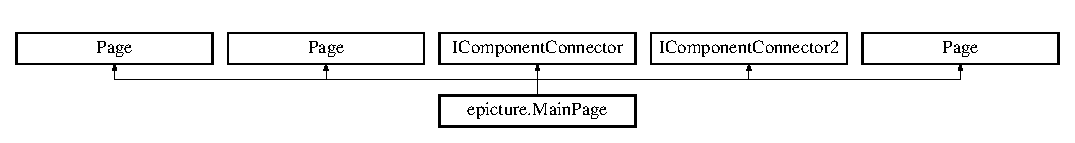
\includegraphics[height=1.473684cm]{classepicture_1_1_main_page}
\end{center}
\end{figure}
\subsection*{Public Member Functions}
\begin{DoxyCompactItemize}
\item 
\mbox{\Hypertarget{classepicture_1_1_main_page_af580ad7f9e7a6bfa7ae0340bf1a9aa76}\label{classepicture_1_1_main_page_af580ad7f9e7a6bfa7ae0340bf1a9aa76}} 
void {\bfseries Flickr\+\_\+\+Connection\+Click} (object sender, Routed\+Event\+Args e)
\item 
\mbox{\Hypertarget{classepicture_1_1_main_page_a34f588b307d9dea1e5b3046b3472e724}\label{classepicture_1_1_main_page_a34f588b307d9dea1e5b3046b3472e724}} 
void {\bfseries login\+Test\+Flickr\+Click} (object sender, Routed\+Event\+Args e)
\item 
\mbox{\Hypertarget{classepicture_1_1_main_page_a592bad2d0242a5c3bdf0da0cd5f05228}\label{classepicture_1_1_main_page_a592bad2d0242a5c3bdf0da0cd5f05228}} 
async void {\bfseries Search\+Tag\+Click} (object sender, Routed\+Event\+Args e)
\item 
\mbox{\Hypertarget{classepicture_1_1_main_page_a24d39b00621dfb70fbbc35088f405f4d}\label{classepicture_1_1_main_page_a24d39b00621dfb70fbbc35088f405f4d}} 
async void {\bfseries Imgur\+\_\+\+Get\+Favorites\+Click} (object sender, Routed\+Event\+Args e)
\item 
\mbox{\Hypertarget{classepicture_1_1_main_page_a52713a040797f1570484213c2d292846}\label{classepicture_1_1_main_page_a52713a040797f1570484213c2d292846}} 
async void {\bfseries Imgur\+\_\+\+Get\+Posts\+Click} (object sender, Routed\+Event\+Args e)
\item 
\mbox{\Hypertarget{classepicture_1_1_main_page_a392e46fadfee49659df5cb66a51d3146}\label{classepicture_1_1_main_page_a392e46fadfee49659df5cb66a51d3146}} 
void {\bfseries Imgur\+\_\+\+Add\+Favoris\+Click} (object sender, Routed\+Event\+Args e)
\item 
\mbox{\Hypertarget{classepicture_1_1_main_page_aba8153d4a3931c63bff8b9106c4b1924}\label{classepicture_1_1_main_page_aba8153d4a3931c63bff8b9106c4b1924}} 
void {\bfseries Imgur\+\_\+\+Delete\+Click} (object sender, Routed\+Event\+Args e)
\item 
\mbox{\Hypertarget{classepicture_1_1_main_page_a40dea502bf70bacc5831aa9979bdb0f3}\label{classepicture_1_1_main_page_a40dea502bf70bacc5831aa9979bdb0f3}} 
void {\bfseries Imgur\+\_\+\+Post\+Click} (object sender, Routed\+Event\+Args e)
\item 
\mbox{\Hypertarget{classepicture_1_1_main_page_ae6731b198334f30de0431b0440f67e71}\label{classepicture_1_1_main_page_ae6731b198334f30de0431b0440f67e71}} 
async void {\bfseries Imgur\+\_\+\+Connection\+Click} (object sender, Routed\+Event\+Args e)
\item 
\mbox{\Hypertarget{classepicture_1_1_main_page_a76553f8ceef4112f3c7dc55d9601e8e4}\label{classepicture_1_1_main_page_a76553f8ceef4112f3c7dc55d9601e8e4}} 
void {\bfseries set\+Text\+Box\+Warning} (string text)
\item 
void \mbox{\hyperlink{classepicture_1_1_main_page_addc532a5876a946b3fa6859fedbe8eb7}{Connect}} (int connection\+Id, object target)
\begin{DoxyCompactList}\small\item\em \mbox{\hyperlink{classepicture_1_1_main_page_addc532a5876a946b3fa6859fedbe8eb7}{Connect()}} \end{DoxyCompactList}\item 
\mbox{\Hypertarget{classepicture_1_1_main_page_ac478279ce6b7d7786558e1c7610bd1ac}\label{classepicture_1_1_main_page_ac478279ce6b7d7786558e1c7610bd1ac}} 
global\+::\+Windows.\+U\+I.\+Xaml.\+Markup.\+I\+Component\+Connector {\bfseries Get\+Binding\+Connector} (int connection\+Id, object target)
\item 
void \mbox{\hyperlink{classepicture_1_1_main_page_ae68560cfe8407bb0ad02d82217f93ef3}{Initialize\+Component}} ()
\begin{DoxyCompactList}\small\item\em \mbox{\hyperlink{classepicture_1_1_main_page_ae68560cfe8407bb0ad02d82217f93ef3}{Initialize\+Component()}} \end{DoxyCompactList}\end{DoxyCompactItemize}
\subsection*{Static Public Attributes}
\begin{DoxyCompactItemize}
\item 
\mbox{\Hypertarget{classepicture_1_1_main_page_ab005e8d0d9e35b69547a00debd7a1cb7}\label{classepicture_1_1_main_page_ab005e8d0d9e35b69547a00debd7a1cb7}} 
static \mbox{\hyperlink{classepicture_1_1_main_page}{Main\+Page}} {\bfseries Current}
\end{DoxyCompactItemize}
\subsection*{Private Attributes}
\begin{DoxyCompactItemize}
\item 
\mbox{\Hypertarget{classepicture_1_1_main_page_a0ee9be5edd32a622d3650cc28bd22069}\label{classepicture_1_1_main_page_a0ee9be5edd32a622d3650cc28bd22069}} 
\mbox{\hyperlink{classepicture_1_1_imgur_api}{Imgur\+Api}} {\bfseries Imgur\+Api}
\item 
\mbox{\Hypertarget{classepicture_1_1_main_page_a1a9b84824af16dcbae10c28555e7c7a7}\label{classepicture_1_1_main_page_a1a9b84824af16dcbae10c28555e7c7a7}} 
\mbox{\hyperlink{classepicture_1_1_flickr_api}{Flickr\+Api}} {\bfseries Flickr\+Api}
\item 
\mbox{\Hypertarget{classepicture_1_1_main_page_adffd553f506a93152a88d075fca2a462}\label{classepicture_1_1_main_page_adffd553f506a93152a88d075fca2a462}} 
global\+::\+Windows.\+U\+I.\+Xaml.\+Controls.\+Text\+Block {\bfseries Text\+Block\+Warning}
\item 
\mbox{\Hypertarget{classepicture_1_1_main_page_a206120cf5027642cff943f1b1ffeba52}\label{classepicture_1_1_main_page_a206120cf5027642cff943f1b1ffeba52}} 
global\+::\+Windows.\+U\+I.\+Xaml.\+Controls.\+Text\+Box {\bfseries Text\+Box\+Tag}
\item 
\mbox{\Hypertarget{classepicture_1_1_main_page_a703be6189a1a0d89a5ab694faef62eb0}\label{classepicture_1_1_main_page_a703be6189a1a0d89a5ab694faef62eb0}} 
global\+::\+Windows.\+U\+I.\+Xaml.\+Controls.\+Text\+Box {\bfseries Text\+Box\+Nb}
\item 
\mbox{\Hypertarget{classepicture_1_1_main_page_a86ba2eb08c9857bf874b20e640ed2b62}\label{classepicture_1_1_main_page_a86ba2eb08c9857bf874b20e640ed2b62}} 
global\+::\+Windows.\+U\+I.\+Xaml.\+Controls.\+Button {\bfseries Button\+Search\+Tag}
\item 
\mbox{\Hypertarget{classepicture_1_1_main_page_aedbb03c5cbc6333fb16dbc2d2e57159d}\label{classepicture_1_1_main_page_aedbb03c5cbc6333fb16dbc2d2e57159d}} 
global\+::\+Windows.\+U\+I.\+Xaml.\+Controls.\+Button {\bfseries Button\+Connect\+Imgur}
\item 
\mbox{\Hypertarget{classepicture_1_1_main_page_a1cb464f71fa6d7d23aea30edd06c324a}\label{classepicture_1_1_main_page_a1cb464f71fa6d7d23aea30edd06c324a}} 
global\+::\+Windows.\+U\+I.\+Xaml.\+Controls.\+Button {\bfseries Button\+Connect\+Flickr}
\item 
\mbox{\Hypertarget{classepicture_1_1_main_page_aefaef431a15018a496f89543b08c028d}\label{classepicture_1_1_main_page_aefaef431a15018a496f89543b08c028d}} 
global\+::\+Windows.\+U\+I.\+Xaml.\+Controls.\+Button {\bfseries Button\+Imgur\+Post}
\item 
\mbox{\Hypertarget{classepicture_1_1_main_page_aa8dc4dfee835aaae949a5a23d83bfb8a}\label{classepicture_1_1_main_page_aa8dc4dfee835aaae949a5a23d83bfb8a}} 
global\+::\+Windows.\+U\+I.\+Xaml.\+Controls.\+Text\+Box {\bfseries Text\+Box\+Post\+File}
\item 
\mbox{\Hypertarget{classepicture_1_1_main_page_acd5b45578884cfdee08899b8c75f8271}\label{classepicture_1_1_main_page_acd5b45578884cfdee08899b8c75f8271}} 
global\+::\+Windows.\+U\+I.\+Xaml.\+Controls.\+Button {\bfseries Button\+Imgur\+Get\+Post}
\item 
\mbox{\Hypertarget{classepicture_1_1_main_page_a8c12009fcfe821c84efdae8adb7e29a3}\label{classepicture_1_1_main_page_a8c12009fcfe821c84efdae8adb7e29a3}} 
global\+::\+Windows.\+U\+I.\+Xaml.\+Controls.\+Button {\bfseries Button\+Imgur\+Delete\+Post}
\item 
\mbox{\Hypertarget{classepicture_1_1_main_page_ab3b5cf1d5e80940653a925a2c0f418d5}\label{classepicture_1_1_main_page_ab3b5cf1d5e80940653a925a2c0f418d5}} 
global\+::\+Windows.\+U\+I.\+Xaml.\+Controls.\+Button {\bfseries Button\+Imgur\+Get\+Favourites}
\item 
\mbox{\Hypertarget{classepicture_1_1_main_page_a9e69e6fc57ee50ab59323c97c37ff076}\label{classepicture_1_1_main_page_a9e69e6fc57ee50ab59323c97c37ff076}} 
global\+::\+Windows.\+U\+I.\+Xaml.\+Controls.\+Button {\bfseries Button\+Imgur\+Add\+Favourites}
\item 
\mbox{\Hypertarget{classepicture_1_1_main_page_aab6beb347ca56d458169b1c59b070fa6}\label{classepicture_1_1_main_page_aab6beb347ca56d458169b1c59b070fa6}} 
global\+::\+Windows.\+U\+I.\+Xaml.\+Controls.\+List\+View {\bfseries List\+View\+Tag\+\_\+\+Imgur}
\item 
\mbox{\Hypertarget{classepicture_1_1_main_page_a28d96d93102a5420fefb1c5a0f38b7d1}\label{classepicture_1_1_main_page_a28d96d93102a5420fefb1c5a0f38b7d1}} 
global\+::\+Windows.\+U\+I.\+Xaml.\+Controls.\+List\+View {\bfseries List\+View\+Tag\+\_\+\+Flickr}
\item 
\mbox{\Hypertarget{classepicture_1_1_main_page_a1b8c972cd834fe801dd3d52ac47a6a4d}\label{classepicture_1_1_main_page_a1b8c972cd834fe801dd3d52ac47a6a4d}} 
bool {\bfseries \+\_\+content\+Loaded}
\end{DoxyCompactItemize}
\subsection*{Static Private Attributes}
\begin{DoxyCompactItemize}
\item 
\mbox{\Hypertarget{classepicture_1_1_main_page_acd0d05d5ed8d0096df5eece5e2ad64b6}\label{classepicture_1_1_main_page_acd0d05d5ed8d0096df5eece5e2ad64b6}} 
static readonly Http\+Client {\bfseries client\+\_\+http} = new Http\+Client()
\end{DoxyCompactItemize}


\subsection{Detailed Description}
Une page vide peut être utilisée seule ou constituer une page de destination au sein d\textquotesingle{}un frame. 



\subsection{Member Function Documentation}
\mbox{\Hypertarget{classepicture_1_1_main_page_addc532a5876a946b3fa6859fedbe8eb7}\label{classepicture_1_1_main_page_addc532a5876a946b3fa6859fedbe8eb7}} 
\index{epicture\+::\+Main\+Page@{epicture\+::\+Main\+Page}!Connect@{Connect}}
\index{Connect@{Connect}!epicture\+::\+Main\+Page@{epicture\+::\+Main\+Page}}
\subsubsection{\texorpdfstring{Connect()}{Connect()}}
{\footnotesize\ttfamily void epicture.\+Main\+Page.\+Connect (\begin{DoxyParamCaption}\item[{int}]{connection\+Id,  }\item[{object}]{target }\end{DoxyParamCaption})}



\mbox{\hyperlink{classepicture_1_1_main_page_addc532a5876a946b3fa6859fedbe8eb7}{Connect()}} 

\mbox{\Hypertarget{classepicture_1_1_main_page_ae68560cfe8407bb0ad02d82217f93ef3}\label{classepicture_1_1_main_page_ae68560cfe8407bb0ad02d82217f93ef3}} 
\index{epicture\+::\+Main\+Page@{epicture\+::\+Main\+Page}!Initialize\+Component@{Initialize\+Component}}
\index{Initialize\+Component@{Initialize\+Component}!epicture\+::\+Main\+Page@{epicture\+::\+Main\+Page}}
\subsubsection{\texorpdfstring{Initialize\+Component()}{InitializeComponent()}}
{\footnotesize\ttfamily void epicture.\+Main\+Page.\+Initialize\+Component (\begin{DoxyParamCaption}{ }\end{DoxyParamCaption})}



\mbox{\hyperlink{classepicture_1_1_main_page_ae68560cfe8407bb0ad02d82217f93ef3}{Initialize\+Component()}} 



The documentation for this class was generated from the following files\+:\begin{DoxyCompactItemize}
\item 
epicture/epicture/Main\+Page.\+xaml.\+cs\item 
epicture/epicture/obj/x86/\+Debug/Main\+Page.\+g.\+i.\+cs\item 
epicture/epicture/obj/x86/\+Debug/Main\+Page.\+g.\+cs\end{DoxyCompactItemize}

%--- End generated contents ---

% Index
\backmatter
\newpage
\phantomsection
\clearemptydoublepage
\addcontentsline{toc}{chapter}{Index}
\printindex

\end{document}
